\section{Calculating the built in potential}  \label{sssec:initial}
The first step to performing a device simulation, is to calculate the built in potential of the device.  To do this we must know the following things:

\begin{itemize}

  \item The majority carrier concentrations on the contacts $n$ and $p$.
  \item The effective densities of states $N_{LUMO}$ and $N_{HOMO}$.
  \item The effective band gap $E_g$

\end{itemize}

\begin{figure}[H]
\centering
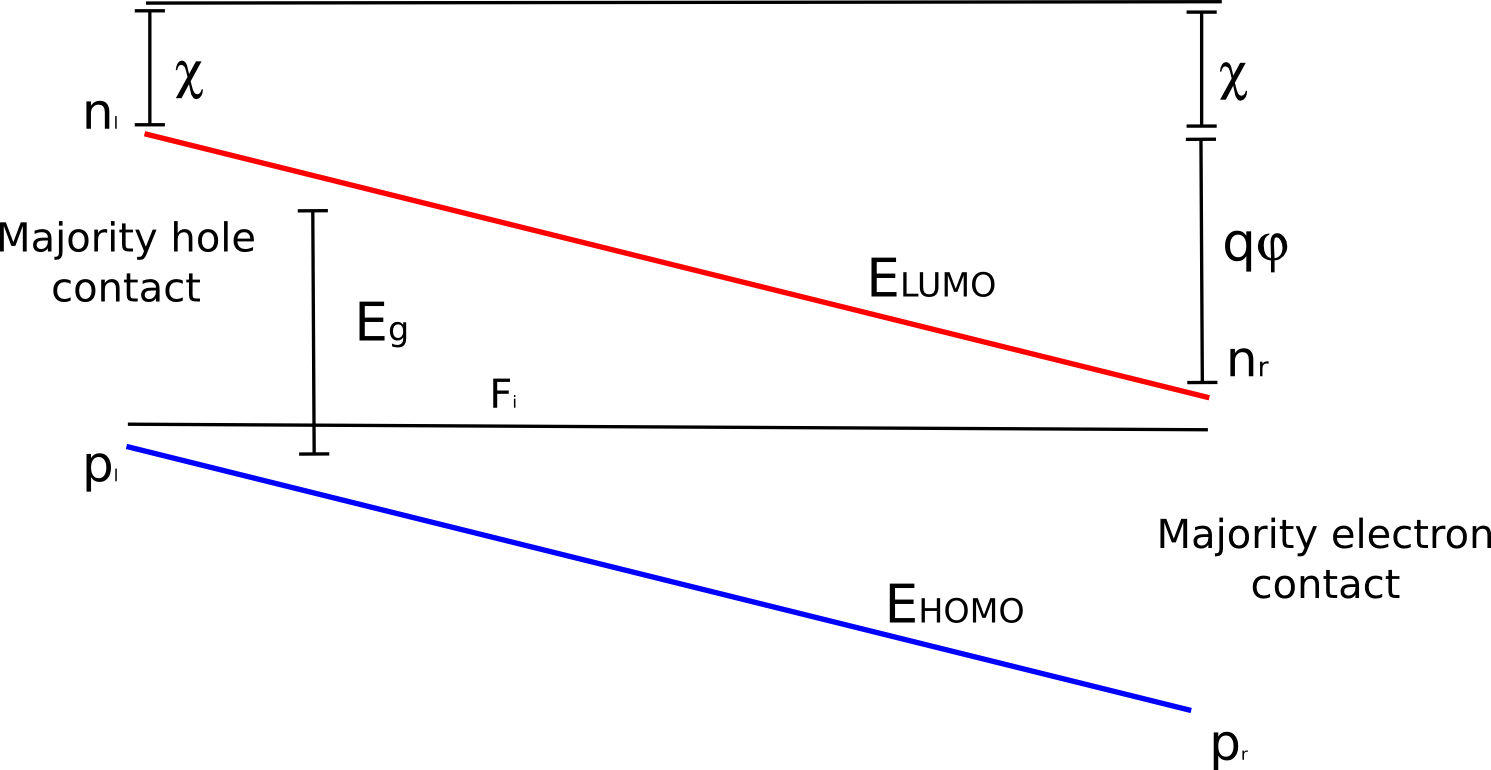
\includegraphics[width=120mm]{./images/bands.png}
\caption{Band structure of device in equilibrium.}
\label{fig:bands}
\end{figure}

\vspace{1em}
The left hand side of the device is given a reference potential of 0 V.  See figure \ref{fig:bands}.  We can then write the energy of the LUMO and HOMO on the left hand side of the device as:

\begin{equation}
E_{LUMO}=-\chi
\end{equation}

\begin{equation}
E_{HOMO}=-\chi-E_{g}
\end{equation}

For the left hand side of the device, we can use Maxwell-Boltzmann statistics to calculate the equilibrium Fermi-level ($F_i$).

\begin{equation}
p_{l}=N_v exp \left(\frac{E_{HOMO}-F_p}{kT} \right)
\end{equation}

We can then calculate the minority carrier concentration on the left hand side using $F_i$

\begin{equation}
n_{l}=N_c exp \left (\frac{F_n-E_{LUMO}}{kT} \right)
\end{equation}

The Fermi-level must be flat across the entire device because it is in equilibrium.  However we know there is a built in potential, we can therefore write the potential of the conduction and valance band on the right hand side of the device in terms of $phi$ to take account of the built in potential.

\begin{equation}
E_{LUMO}=-\chi-q\phi
\label{equ:Ev_rhs}
\end{equation}

\begin{equation}
E_{HOMO}=-\chi-E_g-q\phi
\end{equation}

we can now calculate the potential using

\begin{equation}
n_{r}=N_c exp \left (\frac{F_n-E_{LUMO}}{kT} \right)
\end{equation}
equation \ref{equ:Ev_rhs}.

The minority concentration on the right hand side can now also be calculated using.

\begin{equation}
p_{r}=N_v exp \left (\frac{E_v-F_{HOMO}}{kT} \right)
\end{equation}

The result of this calculation is that we now know the built in potential and minority carrier concentrations on both sides of the device.  Note, infinite recombination velocity on the contacts is assumed.  I have not included finite recombination velocities in the model simply because they would add four more fitting parameters and in my experience I have never needed to use them to fit any experimental data I have come across.

Once this calculation has been performed, we can estimate the potential profile between the left and right hand side of the device, using a linear approximation. From this the charge carrier densities across the device can be guessed.  The guess for potential and carrier densities, is then used to prime the main Newton solver.  Where the real value are calculated.  The Newton solver is described in the next section.

